\section{Deep Reinforcement Learning 1 (Tabular Methods)}
\begin{figure}[!h]
    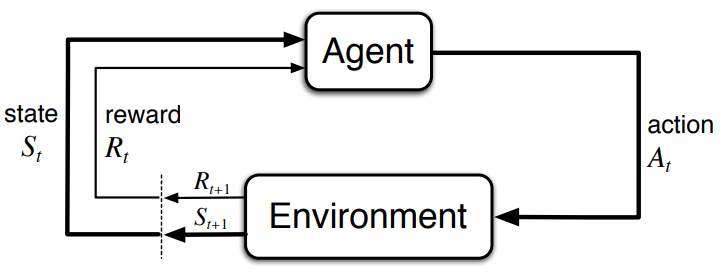
\includegraphics[width = 0.8\columnwidth]{figures/DeepReinforcementLearning1/EnvironmentAgent.png}
\end{figure}

Reinforcement Learning involves an agent interacting with an environment to learn decision-making. The agent:
\begin{itemize}
    \item Takes actions $A_t$ based on states $S_t$.
    \item Receives feedback in the form of rewards $R_t$.
    \item Learns to maximize cumulative rewards (return) $G_t$
\end{itemize}
cumulative reward or return (G):
\[
G_t = R_{t+1} + R_{t+2} + R_{t+3} + \dots + R_T
\]
Discounted return:
\[
G_t = R_{t+1} + \gamma R_{t+2} +\gamma^2 R_{t+3} + \dots = \sum_{k=0}^{\infty}\gamma^k R_{t+k+1}
\]
\begin{figure}[!h]
    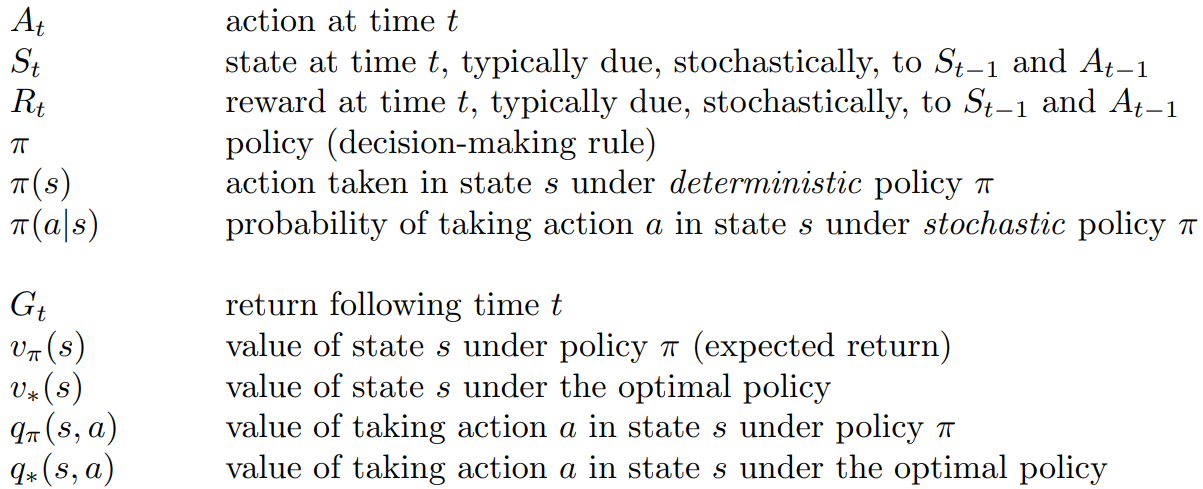
\includegraphics[width = \columnwidth]{figures/DeepReinforcementLearning1/OverviewNotation.png}
\end{figure}
\subsection{Formualtion of the Problem}
\begin{itemize}
    \item The actual value of an action \(a\) is the expected reward (which is not known)
    \[
    q_*(a) = \mathop{\mathbb{E}}[R_t|A_t = a]
    \]
    \item The estimated value of an action is called the (action-) value function \(Q_t(a)\) which we would like to be close to the true value
\end{itemize}
\subsubsection{Action-Value Mehtods}
\begin{itemize}
    \item Simple method(need to keep all rewards):
    \[
    Q_n = \frac{R_1 + R_2 +\dots + R_{n-1}}{n-1}
    \]
    \item Iterativ method:
    \[
    Q_{n+1} = Q_n + \frac{1}{n}(R_n - Q_n)
    \]
    \(R_n - Q_n\)(\(\left[Target- OldEstimation\right]\)) is like a Error.

\end{itemize}
This form
 \[\left[NewEstimation\leftarrow OldEstimation+StepSize\left[Error\right]
\right]\]
with different values for step and Error is used by many RL algorithm.
\subsection{Exploration vs Exploitation}
Exploitation:
\begin{itemize}
    \item Exploit current knowledge by taking  the action with the maximal estimated value
    \item Greedy action
\end{itemize}

Exploration:
\begin{itemize}
    \item Explore the value of other actions to get better estimates
    \item Non greedy actions
\end{itemize}
To balance Exploration and Exploitation:
\begin{itemize}
    \item \textbf{Exploitation:} With probability 1 - \(\epsilon\). Take greedy action with maximal \(Q_t(a)\)(greedy action)
    \item \textbf{Exploration:} With probability \(\epsilon\). Take any valid action with equal probability.
\end{itemize}
To use draw random variable in [0 .. 1].
Compare threshold with \(\epsilon\).
\begin{figure}[]
    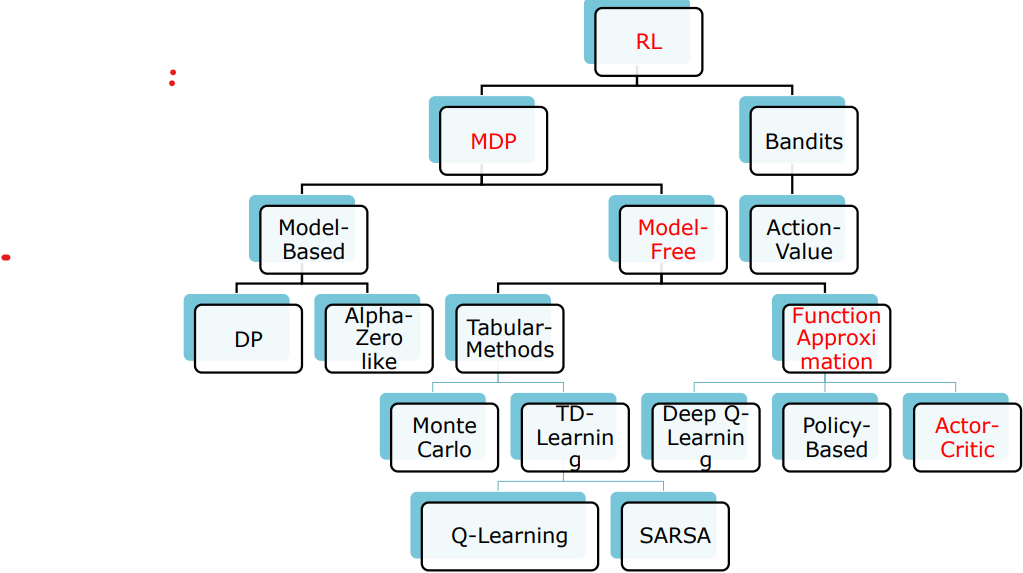
\includegraphics[width = \columnwidth]{figures/DeepReinforcementLearning1/RLOverview.png}
\end{figure}


\subsection{Mehtods Overview}

\subsection{Markov Decision Process (MDP)}
An MDP is defined by:
\begin{itemize}
    \item States $S$, actions $A$, and rewards $R$.
    \item Transition probabilities:
    \[
    p(s', r | s, a) = \Pr\{S_{t+1}=s', R_{t+1}=r | S_t=s, A_t=a\}
    \]
    \item Goal: Maximize the expected cumulative reward.
\end{itemize}

\subsection{Value Functions}
\subsubsection{State and Action-Value Functions}
\begin{itemize}
    \item State-value function under policy $\pi$:
    \[
    v_\pi(s) = \mathbb{E}_\pi[G_t | S_t = s]
    \]
    \item Action-value function under policy $\pi$:
    \[
    q_\pi(s, a) = \mathbb{E}_\pi[G_t | S_t = s, A_t = a]
    \]
\end{itemize}
\subsection{Policies}
A policy is a mapping from states to probabilities of selecting each possible action:
\[
\pi(a|s) = Pr\{A_t = a|S_t = s\}
\]
\subsubsection{Stochastic/Deterministic policies}
\begin{itemize}
    \item \textbf{Stochastic:} Different possible actions with different probabilities for each action. Example: rock, paper, scissor (1/3, 1/3, 1/3)
    \item \textbf{Deterministic:} Single action \(a\) is taken in a state \(s\).
\end{itemize}
\subsubsection{Bellman Equation}
For state-value function:
\[
v_\pi(s) = \sum_a \pi(a|s) \sum_{s', r} p(s', r | s, a) [r + \gamma v_\pi(s')]
\]
\subsection{Calculating the value function}
\begin{itemize}
    \item A solution to the value function for a policy can be found by solving the system of equations given by the Bellman equation for each state.
    \item If there are many states this system becomes large and computationally ineffective to calculate.
    \item We can solve it incrementally using Iterativ Mehtods (Dynammic Programming)
    \item However: Most often we do not have the Markov Decision Process given and have to explore the environment
\end{itemize}

\subsection{RL Algorithms: Value based methods}
\subsubsection{Monte-Carlo methods}
\begin{itemize}
    \item Monte-Carlo (MC) methods look at whole episodes and the average the complete results
    \item The task must be episodic
    \item Value estimations and policies are only changed \textbf{on the completion of an episode}
\end{itemize}

\subsubsection*{Monte Carlo Prediction}
\begin{itemize}
    \item We want to estimate \(v_\pi(s)\), the value of a state \(s\) under the policy \(\pi\).
    \item Given is a set of episodes.
    \item An episode might pass multiple times through\(s\), we will only consider it once, this is known as \textit{first-visit MC}.
    \item We average the retunrs of all episodes
\end{itemize}
\begin{figure}[!h]
    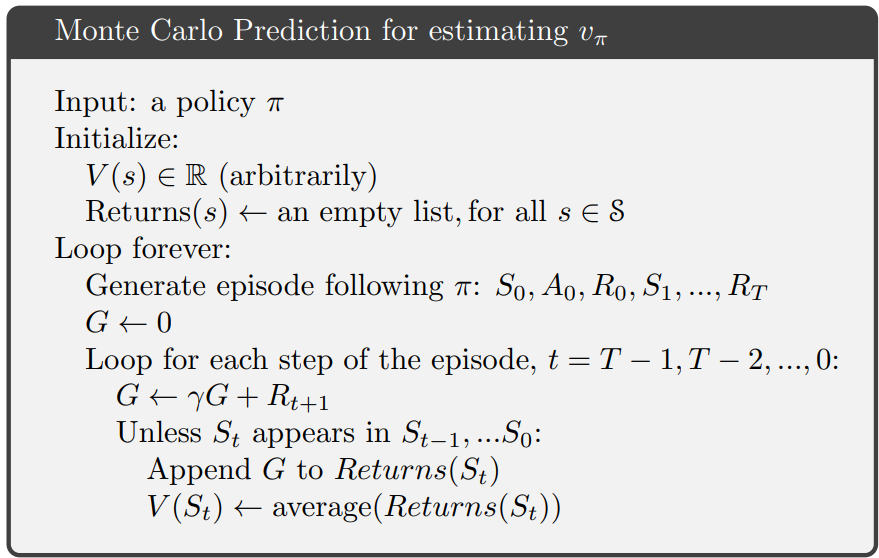
\includegraphics[width = \columnwidth]{figures/DeepReinforcementLearning1/MonteCarlo.png}
    \caption{Monte Carlo Prediction of the State-Value Function (first visit)}
\end{figure}

Intstead of averaging results, we would like an incremental calculation:
\[
    V(S_t) \leftarrow V(S_t) + \alpha[G_t - V(S_t)]
\]
If step size \(\alpha\) is \({1}/{n}\) its the same as averaging.

\subsubsection*{Policy Iteration:}
\begin{itemize}
    \item Knowing the state-value function will not help us to find a better policy, as we do not know which action will generate better returns
    \item Instead, we would like to predict the action-value function Q
    \item Given Q,we can find an improved policy by using greedy actions from Q 
    \item Using the new policy, we can predict its action-value function and repeat
    \item This is known as (generalized) policy-Iteration
\end{itemize}
\begin{figure}[!h]
    \centering
    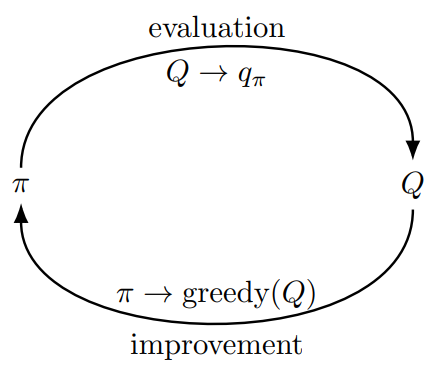
\includegraphics[width = 0.5\columnwidth]{figures/DeepReinforcementLearning1/PolicyIterationMonteCarlo.png}
\end{figure}

\subsubsection*{Exploration in MC}
\begin{itemize}
    \item We must maintain exploration to ensure that all state/action values are visited
    \item Out policy must be epsilon-soft:
    \item Each action in state must occur with a probability grater than zero
    \item 
\end{itemize}
\subsubsection{Temporal Difference (TD) Learning}
\begin{itemize}
    \item MC prediction with constant step size
    \[
    V(S_t) \leftarrow V(S_t) + \alpha[G_t - V(S_t)]
    \]

    \item TD methods make the update immediatly based on the estimates for the next state, which is just the application of the Bellman equation
    \[
    V(S_t) \leftarrow V(S_t) + \alpha[R_{t+1} + \gamma V(S_{t+1}) - V(S_t)]
    \]
\end{itemize}

\subsubsection*{SARSA (On-Policy TD Control)}
\begin{itemize}
    \item We use generalized policy iteration (GPI) for the control problem
    \item As in MC methods, we must balance exploration and exploitation 
    \item TD control methods generally learn an action-value function instead of a state-value function
    \item We look at the transition from (\textbf{S},\textbf{A}) with reward (\textbf{R}) to the next (\textbf{S},\textbf{A})(SARSA)
\end{itemize}
\[
Q(S_t, A_t) \leftarrow Q(S_t, A_t) + \alpha[R_{t+1} + \gamma Q(S_{t+1}, A_{t+1}) - Q(S_t, A_t)]
\]

\subsubsection*{Q-Learning (Off-Policy Control)}
\begin{itemize}
    \item SARSA uses teh Q-Values from the actual Action taken in the next step
    \item This action might not be the one, that maximizes the return
    \item While we cannot change the action taken, we can update the Action-Value using the best (or greedy) action from the next state, this is Q-Learning
\end{itemize}
\[
Q(S_t, A_t) \leftarrow Q(S_t, A_t) + \alpha[R_{t+1} + \gamma \max_a Q(S_{t+1}, a) - Q(S_t, A_t)]
\]
\begin{itemize}
    \item Q-Learning directly tries to approximate the optimal action-value function
    \item It uses a \textbf{soft policy} to determine which actions to take during the episode and the \textbf{greedy policy} to update the action-value estimates
    \item It is called a \textbf{off-policy} algorithm
\end{itemize}
\subsubsection*{Adaptaion}
\begin{itemize}
    \item \textbf{n-Step TD Prediction:} Instead of taking one step and then update the Q-Values we could take 2 or more Steps
    \item \textbf{Lamda-Returns:} Lamda-returns use a weighted sum of all the returns for the estimation
    \[
    G_t^\lambda = (1-\lambda)\sum_{n=1}^{\infty}\lambda^{n-1}G_{t:t+n}
    \]
\end{itemize}
\subsubsection{Summary value based methods}
\textbf{Monte Carlo Estimate:}
\begin{itemize}
    \item Calulate from one episode, estimate is sum of reward
    \item Multiple episode might go through the same state, the MC estimate is the average of those
    \item Estimate have \textbf{high variance}, as the estimates involve many (random) processes and decision along the entire episode
    \item They are \textbf{unbiased}
\end{itemize}
\subsubsection*{TD Estimate:}
\begin{itemize}
    \item A single reward is used and the estimate of the expected return from the next state (the estimate is using another estimate)
    \item Estimates of the next state will not be accurate early in the training
    \item Low variance, as you only depend on the next Steps
    \item Biased, because the estimate depends on the estimate of the next step, which might be inaccurate
\end{itemize}




